\documentclass[14pt,fleqn]{extarticle}
\RequirePackage{prepwell}
\previewoff
\begin{document}


\newcommand\sine{\sin \left( \log x + \phi \right) }
\newcommand\cosine{\cos \left( \log x + \phi \right)}
\newcommand\scos{\cos \left(\log x \right) }
\newcommand\ssin{\sin \left(\log x \right) }

%text
If $y = 3\cdot \cos \left(\log x \right) + 4\cdot \sin \left(\log x \right)$, then show 
that \[ \qquad \qquad x^2\cdot \frac{d^2 y}{dx^2} + x\cdot \frac{dy}{dx} + y = 0 \]
%

\newcard 

\begin{align}
	y &= 3\cdot \cos \left(\log x \right) + 4\cdot \sin \left(\log x \right) \\ 
	&= N\cdot \left[\frac{3}{N} \cdot \cos \left(\log x \right) + \frac{4}{N}\cdot \sin \left(\log x \right) \right] \\
	&= N\cdot \sine  \\
	\text{where } N &= 5,\,\sin\phi = \frac{3}{5}\text{ and } \cos\phi = \frac{4}{5}
\end{align}

\newcard 

Notice that $3^2 + 4^2 = 5^2$. Hence, if there were a triangle such as the one below 

\begin{center} 
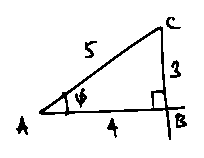
\includegraphics[scale=1.7]{figure.eps} 
\end{center} 

then $\cos\phi = \frac{4}{5}$ and $\sin\phi = \frac{3}{5}$. And hence, 

\begin{align}
	y &= 5 \left[\frac{3}{5}\scos  + \frac{4}{5} \ssin \right] \\
	&= 5 \underbrace{\left[\sin\phi \cdot \scos + \cos\phi\cdot \ssin \right]}_{\sin A\cos B + \cos A\sin B = \sin \left(A+B \right)} \\
	&= 5 \cdot \sine 
\end{align}

So, instead of two trigonometric terms -- $\scos$ and $\ssin$ -- we now have just one -- $\sine$ -- in $y$. Should make life easier! 

\newcard 

\begin{align}
y &= 5 \sine \\ 
y' &= \frac{dy}{dx} = \frac{5}{x} \cosine \\
y'' &= \frac{d^2 y}{dx^2} = -\frac{5}{x^2} \left[ \sine + \cosine \right]
\end{align}

\newcard 

\begin{align}
y &= 5 \sine \\ 
y' &= \frac{dy}{dx} = 5\cdot\cosine \\ 
y'' &= \frac{d^2 y}{dx^2} = \frac{5}{x^2} \left[x\cdot\sine + \cosine \right]
\end{align}


\newcard 

\begin{align}
y &= 5 \cdot \sine \\
\therefore y' &= 5\cdot\frac{d}{dx}\sine \\
&= 5 \underbrace{\left[\cosine\cdot \frac{d}{dx} \left(\log x + \phi \right) \right]}_{\text{Chain Rule. $\phi$ is a constant}} \\ 
&= 5\cdot \frac{\cosine}{x} \\
y'' &= 5 \underbrace{\left[ \dfrac{x\cdot \frac{d}{dx}\cosine - \cosine\cdot 1}{x^2}\right]}_{\text{Quotient Rule}} \\
&= 5 \left[ \frac{\overbrace{-\frac{x}{x}\cdot \sine}^{\text{Chain Rule}} -\cosine}{x^2}\right] \\
&= -\frac{5}{x^2} \left[\sine + \cosine \right]
\end{align}

\newcard 

\begin{align}
y'' &= 	-\frac{5}{x^2} \left[\sine + \cosine \right] \\
&= -\frac{y}{x^2} - \frac{y'}{x}  \quad\text{ (hence proved) }
\end{align}

\newcard 
\begin{align}
y'' &= 	-\frac{5}{x^2} \left[\sine + \cosine \right] \\
&= -\frac{\overbrace{5\cdot\sine}^{ y}}{x^2} -\frac{1}{x}\cdot \underbrace{\left[ \frac{5\cdot\cosine}{x}\right]}_{y'} \\
&= -\frac{y}{x^2} -\frac{y'}{x} \implies x^2\cdot y'' + x\cdot y' + y = 0
\end{align}

Hence proved !

\end{document}